\pdfminorversion=4
\documentclass[center]{beamer}
\usepackage[T1]{fontenc}
\usepackage[absolute, overlay]{textpos}
\usepackage{graphicx}
\DeclareGraphicsExtensions{.png, .jpg, .pdf}
\usepackage{hyperref}
\usepackage{url}
\usepackage[version=3]{mhchem}
\usepackage{chemarrow}
\usepackage{multirow}
\usepackage{array}
\usepackage{setspace}
\usepackage{calc}
\usepackage{tcolorbox}
\usepackage[numbers]{natbib}
\usepackage{tikz}
\usetikzlibrary{arrows, shapes, decorations, positioning}
\tcbuselibrary{skins}

%Helvetica sans-serif font
\renewcommand{\sfdefault}{phv}
%Utopia serif font
\renewcommand{\rmdefault}{put}
%\usepackage[quiet]{fontspec}
%\defaultfontfeatures{Ligatures=TeX}
%\setmainfont{Tahoma}
%\setsansfont{Tahoma}

\renewcommand*{\bibfont}{\footnotesize}
\def\newblock{\hskip .11em plus .33em minus .07em}
\newcolumntype{P}[1]{>{\raggedright\let\newline\\\arraybackslash}p{#1}}
\newcolumntype{M}[1]{>{\raggedright\arraybackslash}m{#1}}

\definecolor{TitleBlue}{RGB}{75,151,182}
\definecolor{TextGrey}{RGB}{101,98,99}
\definecolor{BkgdBlue}{RGB}{224,238,244}
\definecolor{BkgdGrey}{RGB}{236,236,236}

\TPGrid[22mm,22mm]{100}{30}

%create colourbox for framing each sections text
\newtcolorbox{BlueBox}{spartan, colback=BkgdBlue, colframe=TitleBlue, toprule=5mm, bottomrule=0mm, rightrule=0mm, leftrule=0mm} %blue boxes
\newtcolorbox{GreyBox}{spartan, colback=white, colframe=TitleBlue, toprule=5mm, bottomrule=1mm, rightrule=1mm, leftrule=1mm} %grey boxes
\newtcolorbox{WhiteBox}{spartan, colback=white, colframe=TextGrey, toprule=5mm, bottomrule=0mm, rightrule=0mm, leftrule=0mm} %footer boxed
\newtcolorbox{ClearBox}{spartan, colback=white, colframe=white, toprule=0mm, bottomrule=0mm, rightrule=0mm, leftrule=0mm} %qr-code boxed

%sizes for different sections
\def\BHead#1{\begin{flushleft}{{\fontseries{bx}\fontsize{40}{44}\selectfont\color{TitleBlue} #1}}\smallskip\end{flushleft}}
\def\GHead#1{\begin{flushleft}{{\fontseries{bx}\fontsize{40}{44}\selectfont\color{TextGrey} #1}}\smallskip\end{flushleft}}
\def\Subhead#1{\noindent{\large\color{white}#1}}
\def\Subsubhead#1{\noindent{\begin{flushleft}{{\fontseries{bx}\fontsize{40}{44}\selectfont\color{TextGrey} #1}}\smallskip\end{flushleft}}}

\hypersetup{pdfauthor = {Jane Coates},
		    pdftitle = {2015 AGU Fall Meeting Poster Presentation},	
		    pdfsubject = {AGU Fall Meeting, tropospheric ozone, temperature, NOx conditions},
		    pdfkeywords = {tropospheric ozone, AGU, temperature, NOx gradients},
            pdfcreator = {Latex with hyperref}}

\setbeamertemplate{navigation symbols}{}
\setbeamercolor{itemize item}{fg=TitleBlue}
\setbeamercolor{local structure}{fg=TitleBlue}
%bibliography
\setbeamercolor{bibliography item}{fg=black}
\setbeamercolor{bibliography entry author}{fg=black}
\setbeamercolor*{bibliography entry title}{fg=black}
\setbeamercolor*{bibliography entry location}{fg=black}
\setbeamercolor*{bibliography entry note}{fg=black}
\setbeamertemplate{bibliography item}[text]

\newcommand{\cemph}[1]{\textcolor{\highlightcolor}{#1}}
\newcommand{\highlightcolor}{TitleBlue}
\newcommand{\authorname}{Jane Coates and Tim Butler}
\newcommand{\postertitle}{The Influence of Atmospheric Conditions on the Production of Ozone during VOC Oxidation}
%\newcommand{\subposter}{Production of Ozone during VOC Oxidation}
\newcommand{\Institute}{Institute for Advanced Sustainability Studies (IASS)}

%header


\begin{document}
{
    \usebackgroundtemplate{%
        \vbox to \paperheight{\vfil\hbox to \paperwidth{\hfil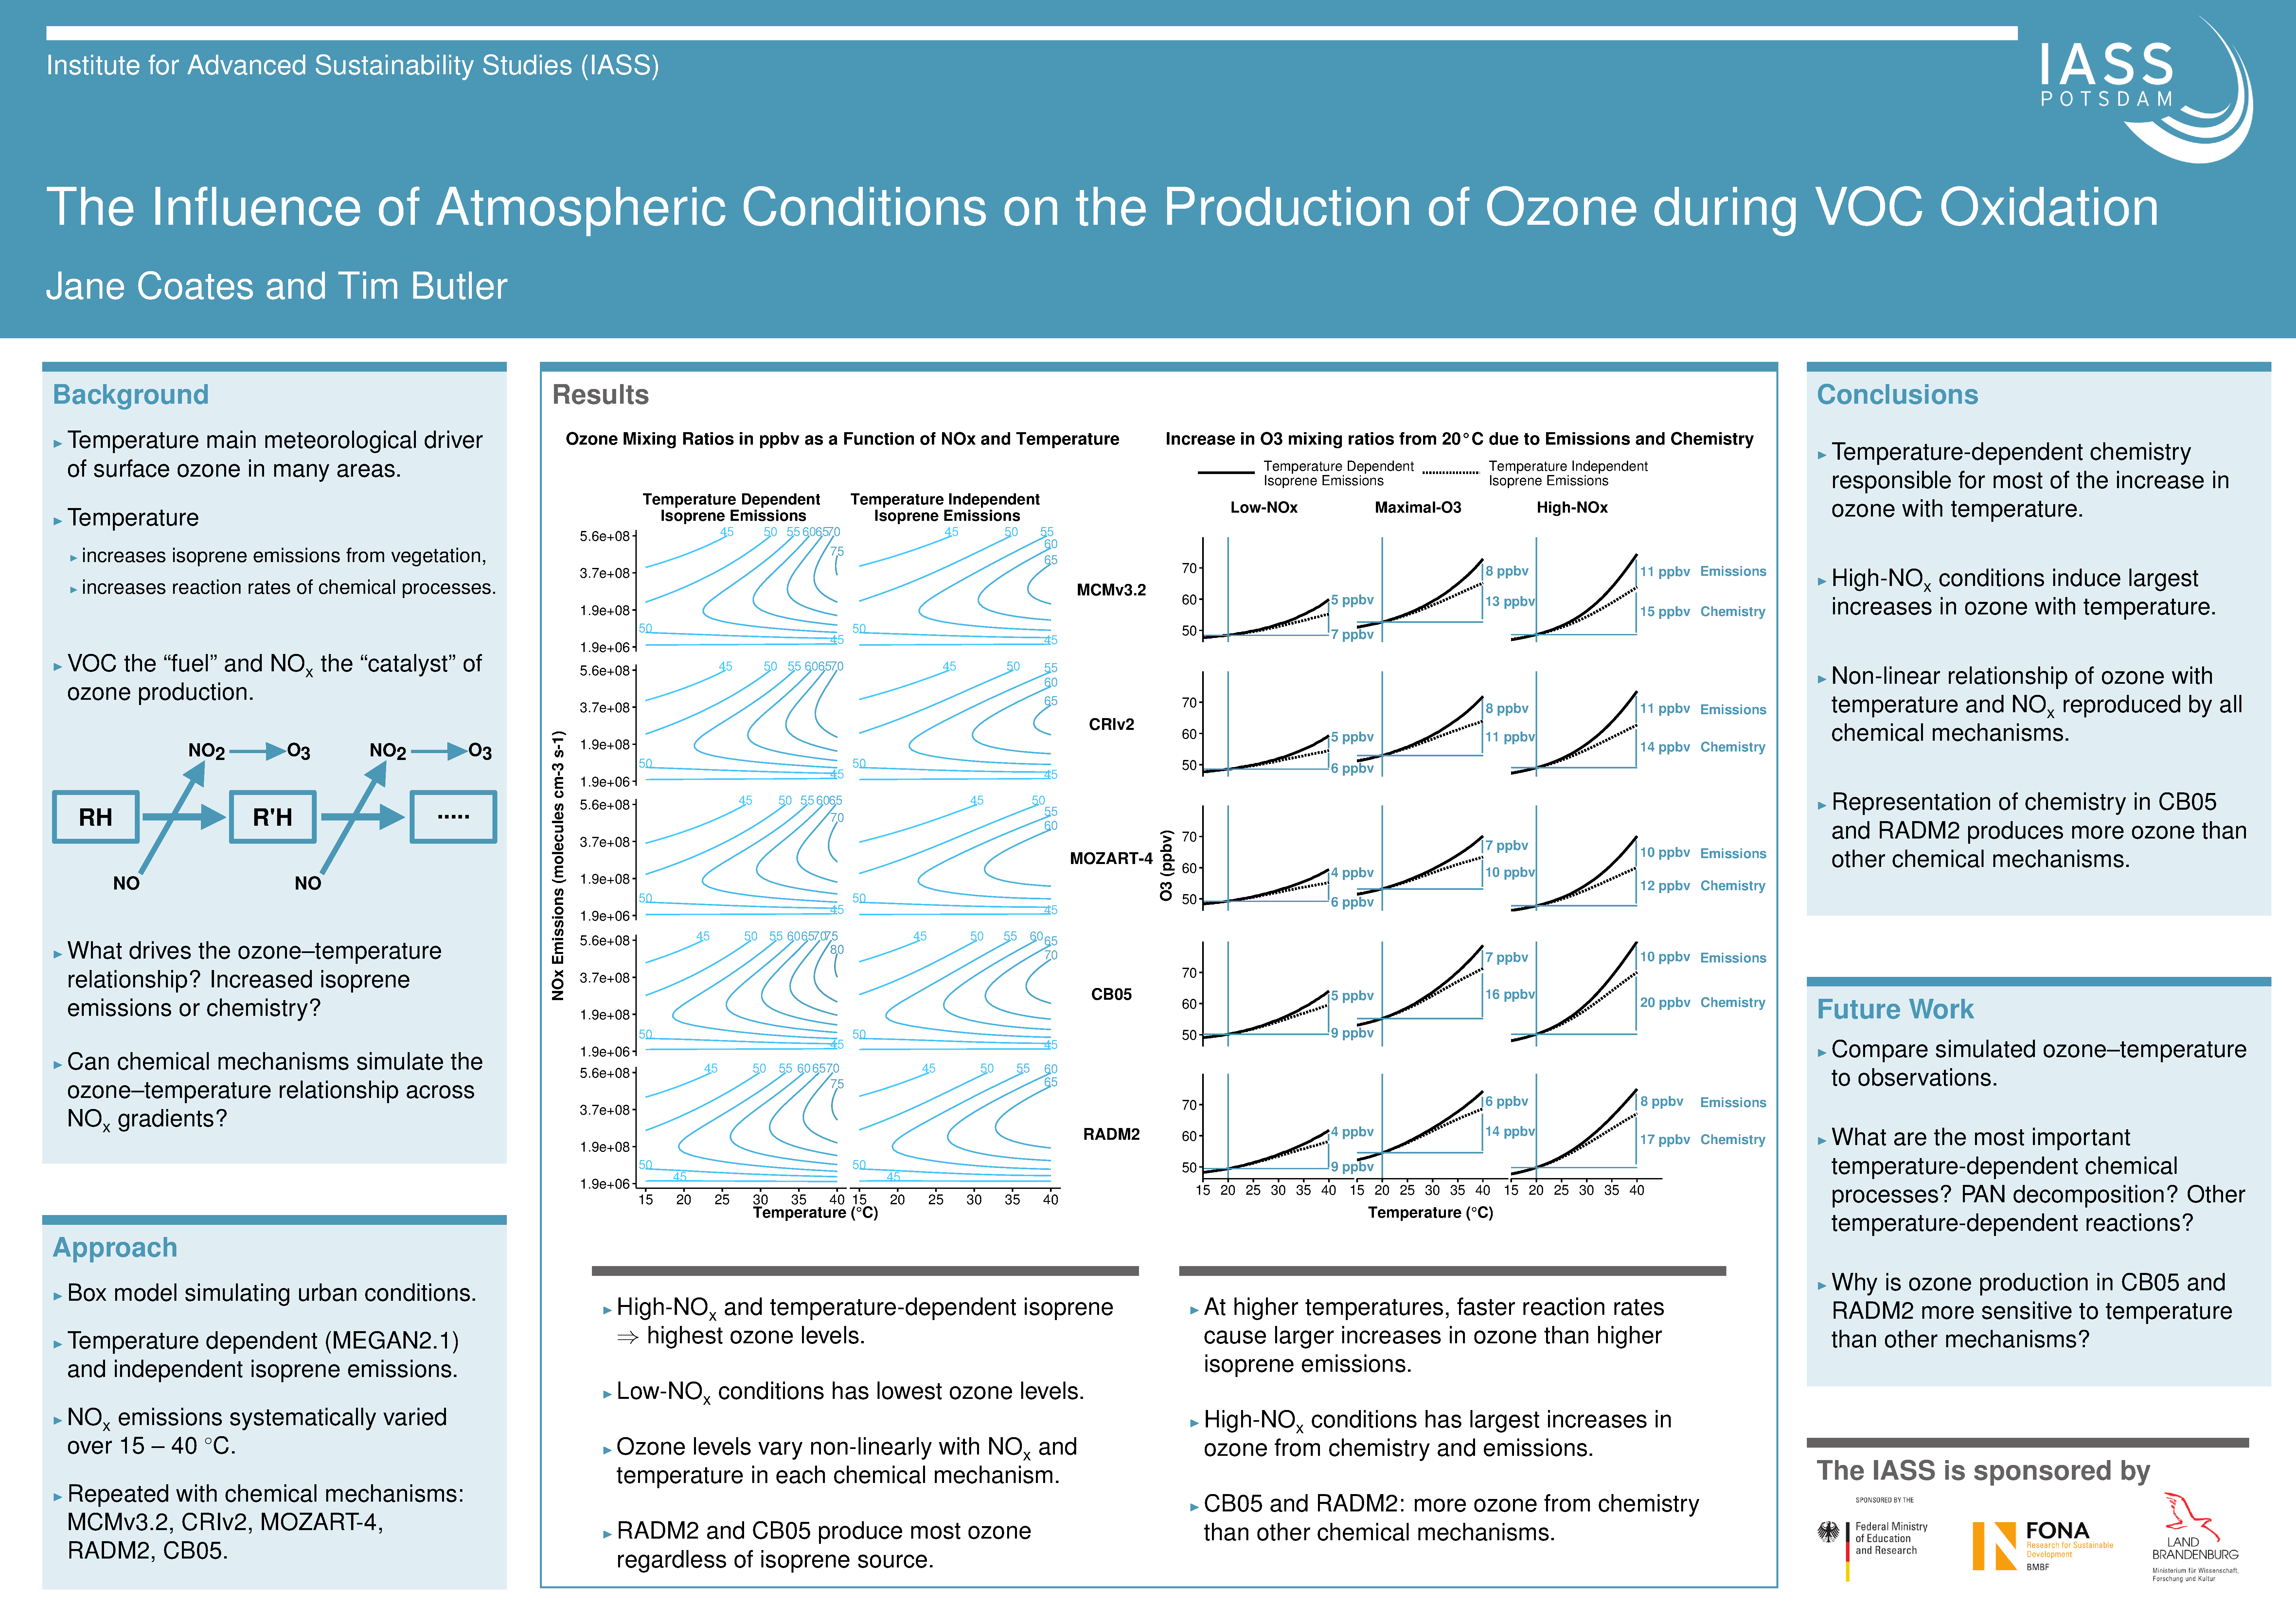
\includegraphics[height = 0.98\paperheight, width = 0.98\paperwidth]{../poster}\hfil}\vfil}
    }
    \begin{frame}[plain]
    \end{frame}
}

{
    \usebackgroundtemplate{%
        \vbox to \paperheight{\vfil\hbox to \paperwidth{\hfil\includegraphics[height = 0.98\paperheight]{background}\hfil}\vfil}
    }
    \begin{frame}[plain]
    \end{frame}
}

{
    \usebackgroundtemplate{%
        \vbox to \paperheight{\vfil\hbox to \paperwidth{\hfil\includegraphics[scale = 0.4]{approach}\hfil}\vfil}
    }
    \begin{frame}[plain]
    \end{frame}
}

{
    \begin{frame}[plain]
        \vspace{-5mm}
        \begin{columns}[onlypaperwidth]
            \begin{column}{0.75\textwidth}
                \begin{center}
                    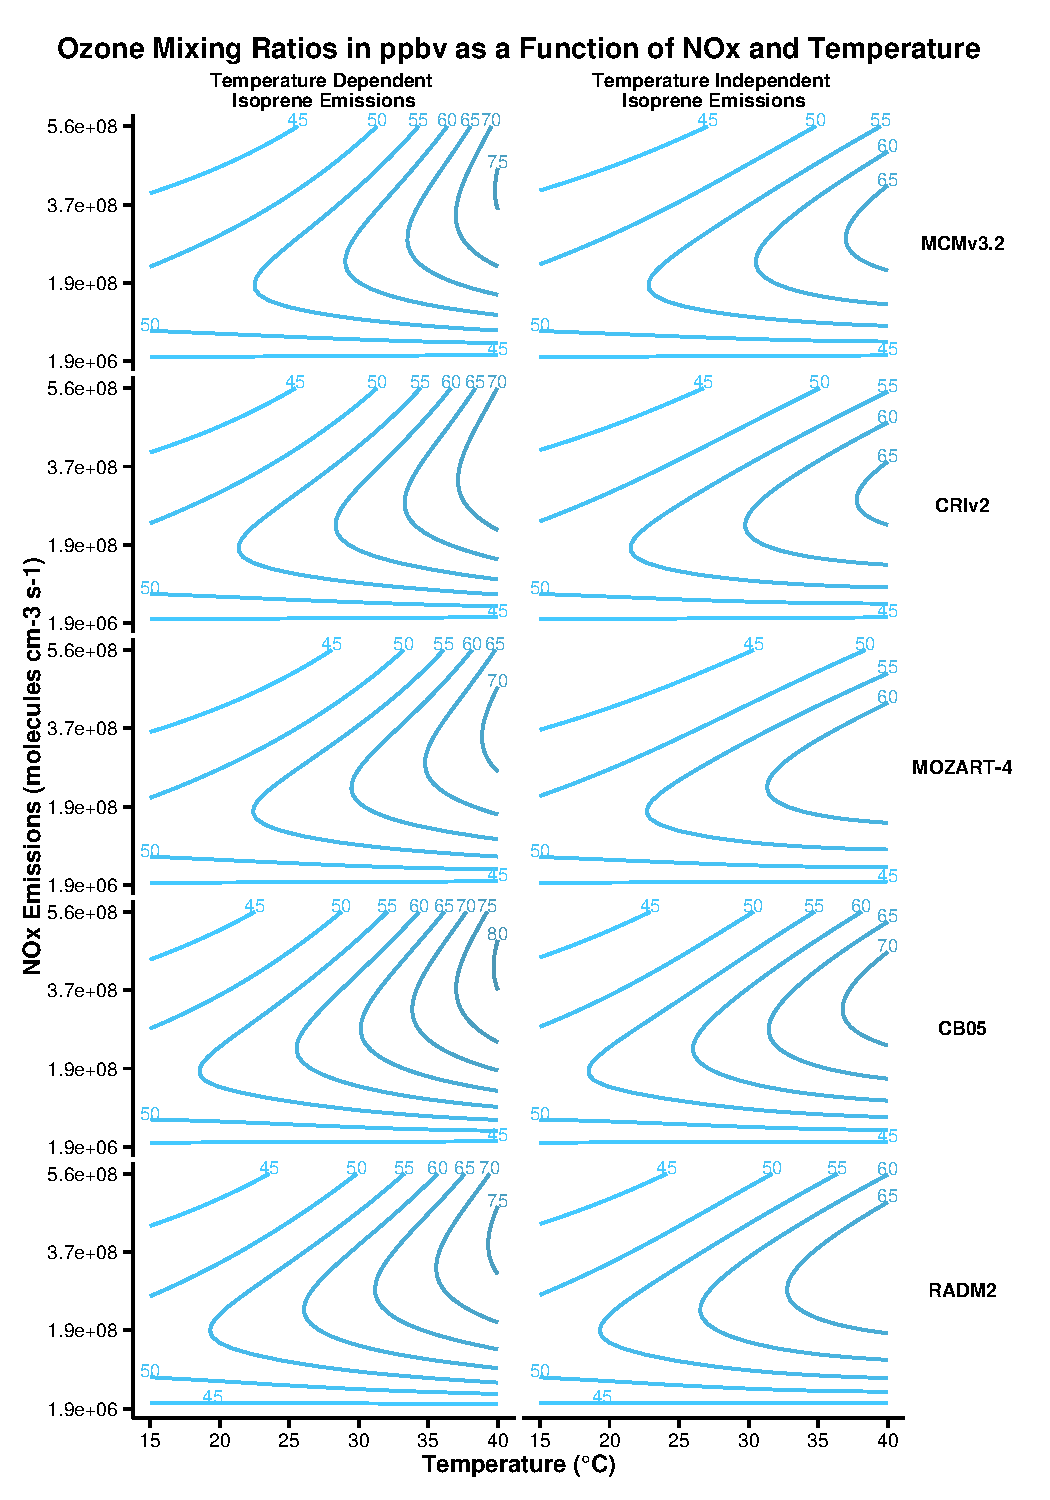
\includegraphics[height = 0.98\paperheight, width = \textwidth]{../Plotting/O3_comparison} 
                \end{center}
            \end{column}%
            \begin{column}{0.43\textwidth} 
                \begin{flushleft}
                    \small{
                        \begin{itemize} 
                            \item High-\ce{NO_x} and temperature-dependent isoprene \\ $\Rightarrow$ highest ozone levels. \vspace{3mm}
                            \item Low-\ce{NO_x} conditions has lowest ozone levels. \vspace{3mm}
                            \item Ozone levels vary non-linearly with \ce{NO_x} and temperature in each chemical mechanism. \vspace{3mm}
                            \item RADM2 and CB05 produce most ozone regardless of isoprene source. %\vspace{13mm}
                        \end{itemize} }
                \end{flushleft}
            \end{column}
        \end{columns}
    \end{frame}
}

{
    \begin{frame}[plain]
        \vspace{-3mm}
        \begin{columns}[onlypaperwidth]
            \begin{column}{0.75\textwidth}
                \begin{center}
                    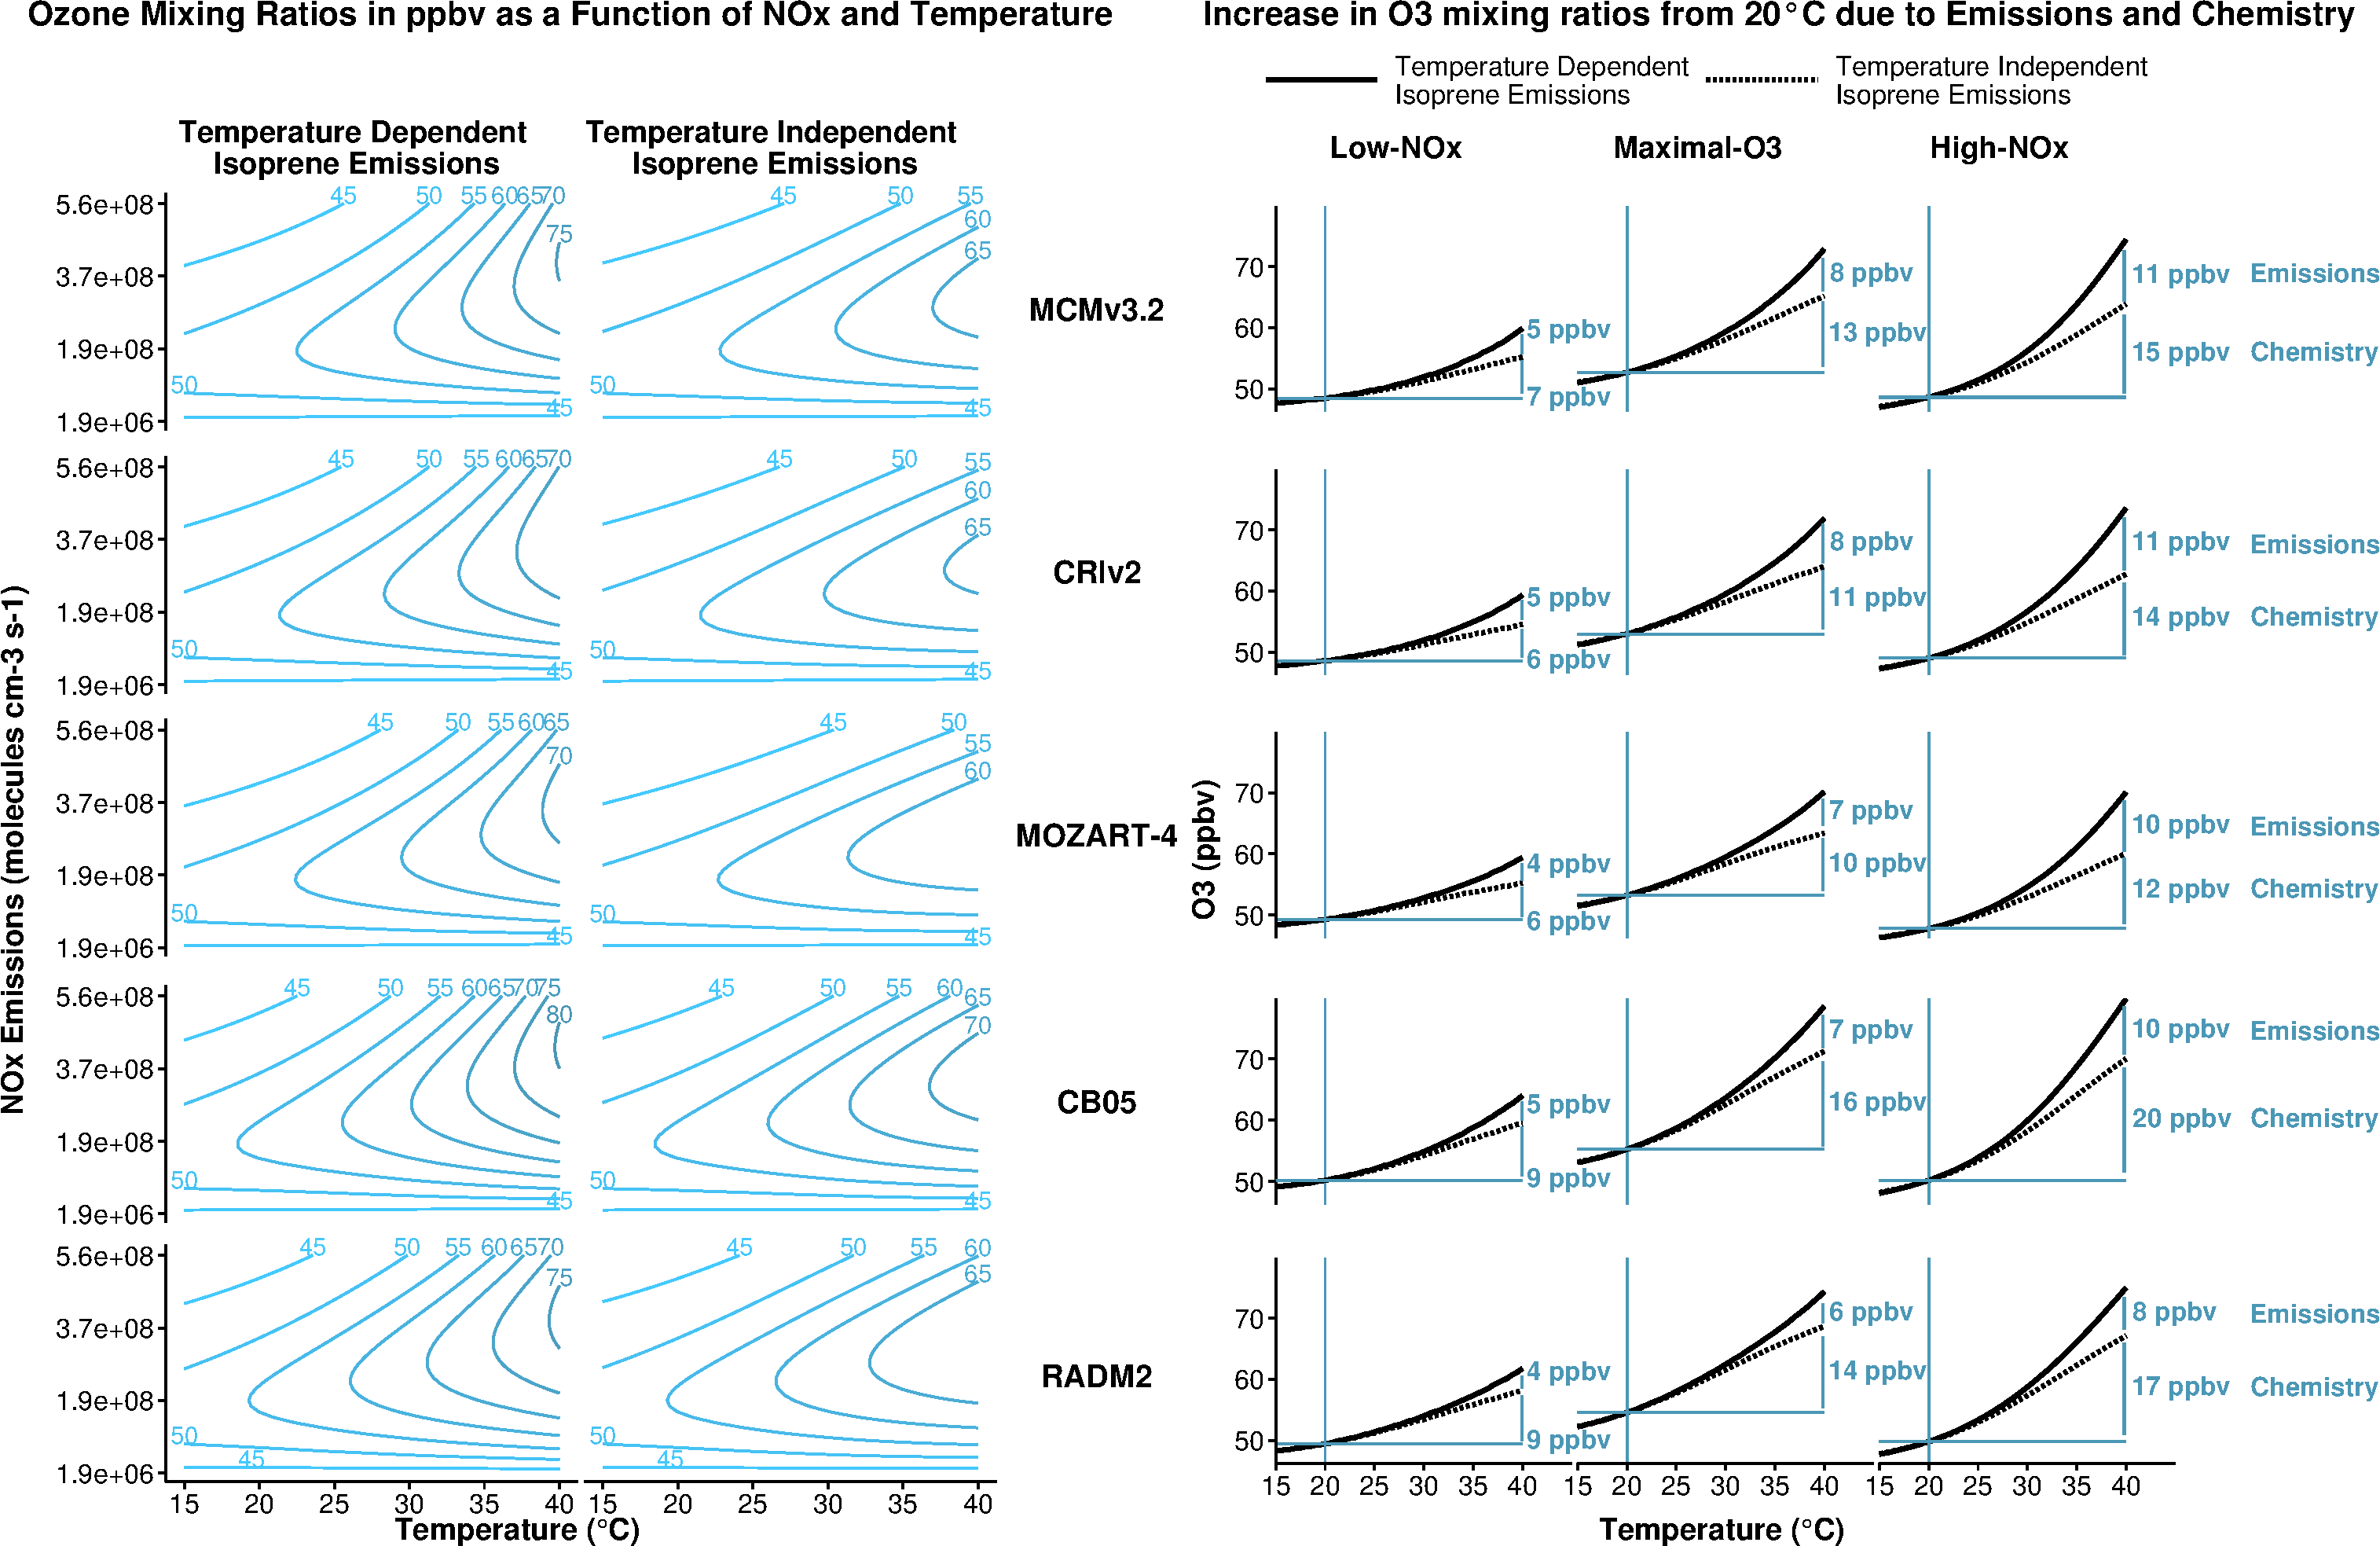
\includegraphics[height = 0.9\paperheight, width = \textwidth]{results} 
                \end{center}
            \end{column}%
            \begin{column}{0.43\textwidth} 
                \begin{flushleft}
                    \small{
                        \begin{itemize} 
                            \item At higher temperatures, faster reaction rates cause larger increases in ozone than higher isoprene emissions. \vspace{3mm}
                            \item High-\ce{NO_x} conditions has largest increases in ozone from chemistry and emissions. \vspace{3mm}
                            \item Increased isoprene emissions in CB05 and RADM2 produces less ozone than other chemical mechanisms. %\vspace{13mm} 
                        \end{itemize} }
                \end{flushleft}
            \end{column}
        \end{columns}
    \end{frame}
}

{
    \usebackgroundtemplate{%
        \vbox to \paperheight{\vfil\hbox to \paperwidth{\hfil\includegraphics[height = 0.98\paperheight]{conclusions}\hfil}\vfil}
    }
    \begin{frame}[plain]
    \end{frame}
}

{
    \usebackgroundtemplate{%
        \vbox to \paperheight{\vfil\hbox to \paperwidth{\hfil\includegraphics[scale = 0.37]{future_work}\hfil}\vfil}
    }
    \begin{frame}[plain]
    \end{frame}
}

{
    \usebackgroundtemplate{%
        \vbox to \paperheight{\vfil\hbox to \paperwidth{\hfil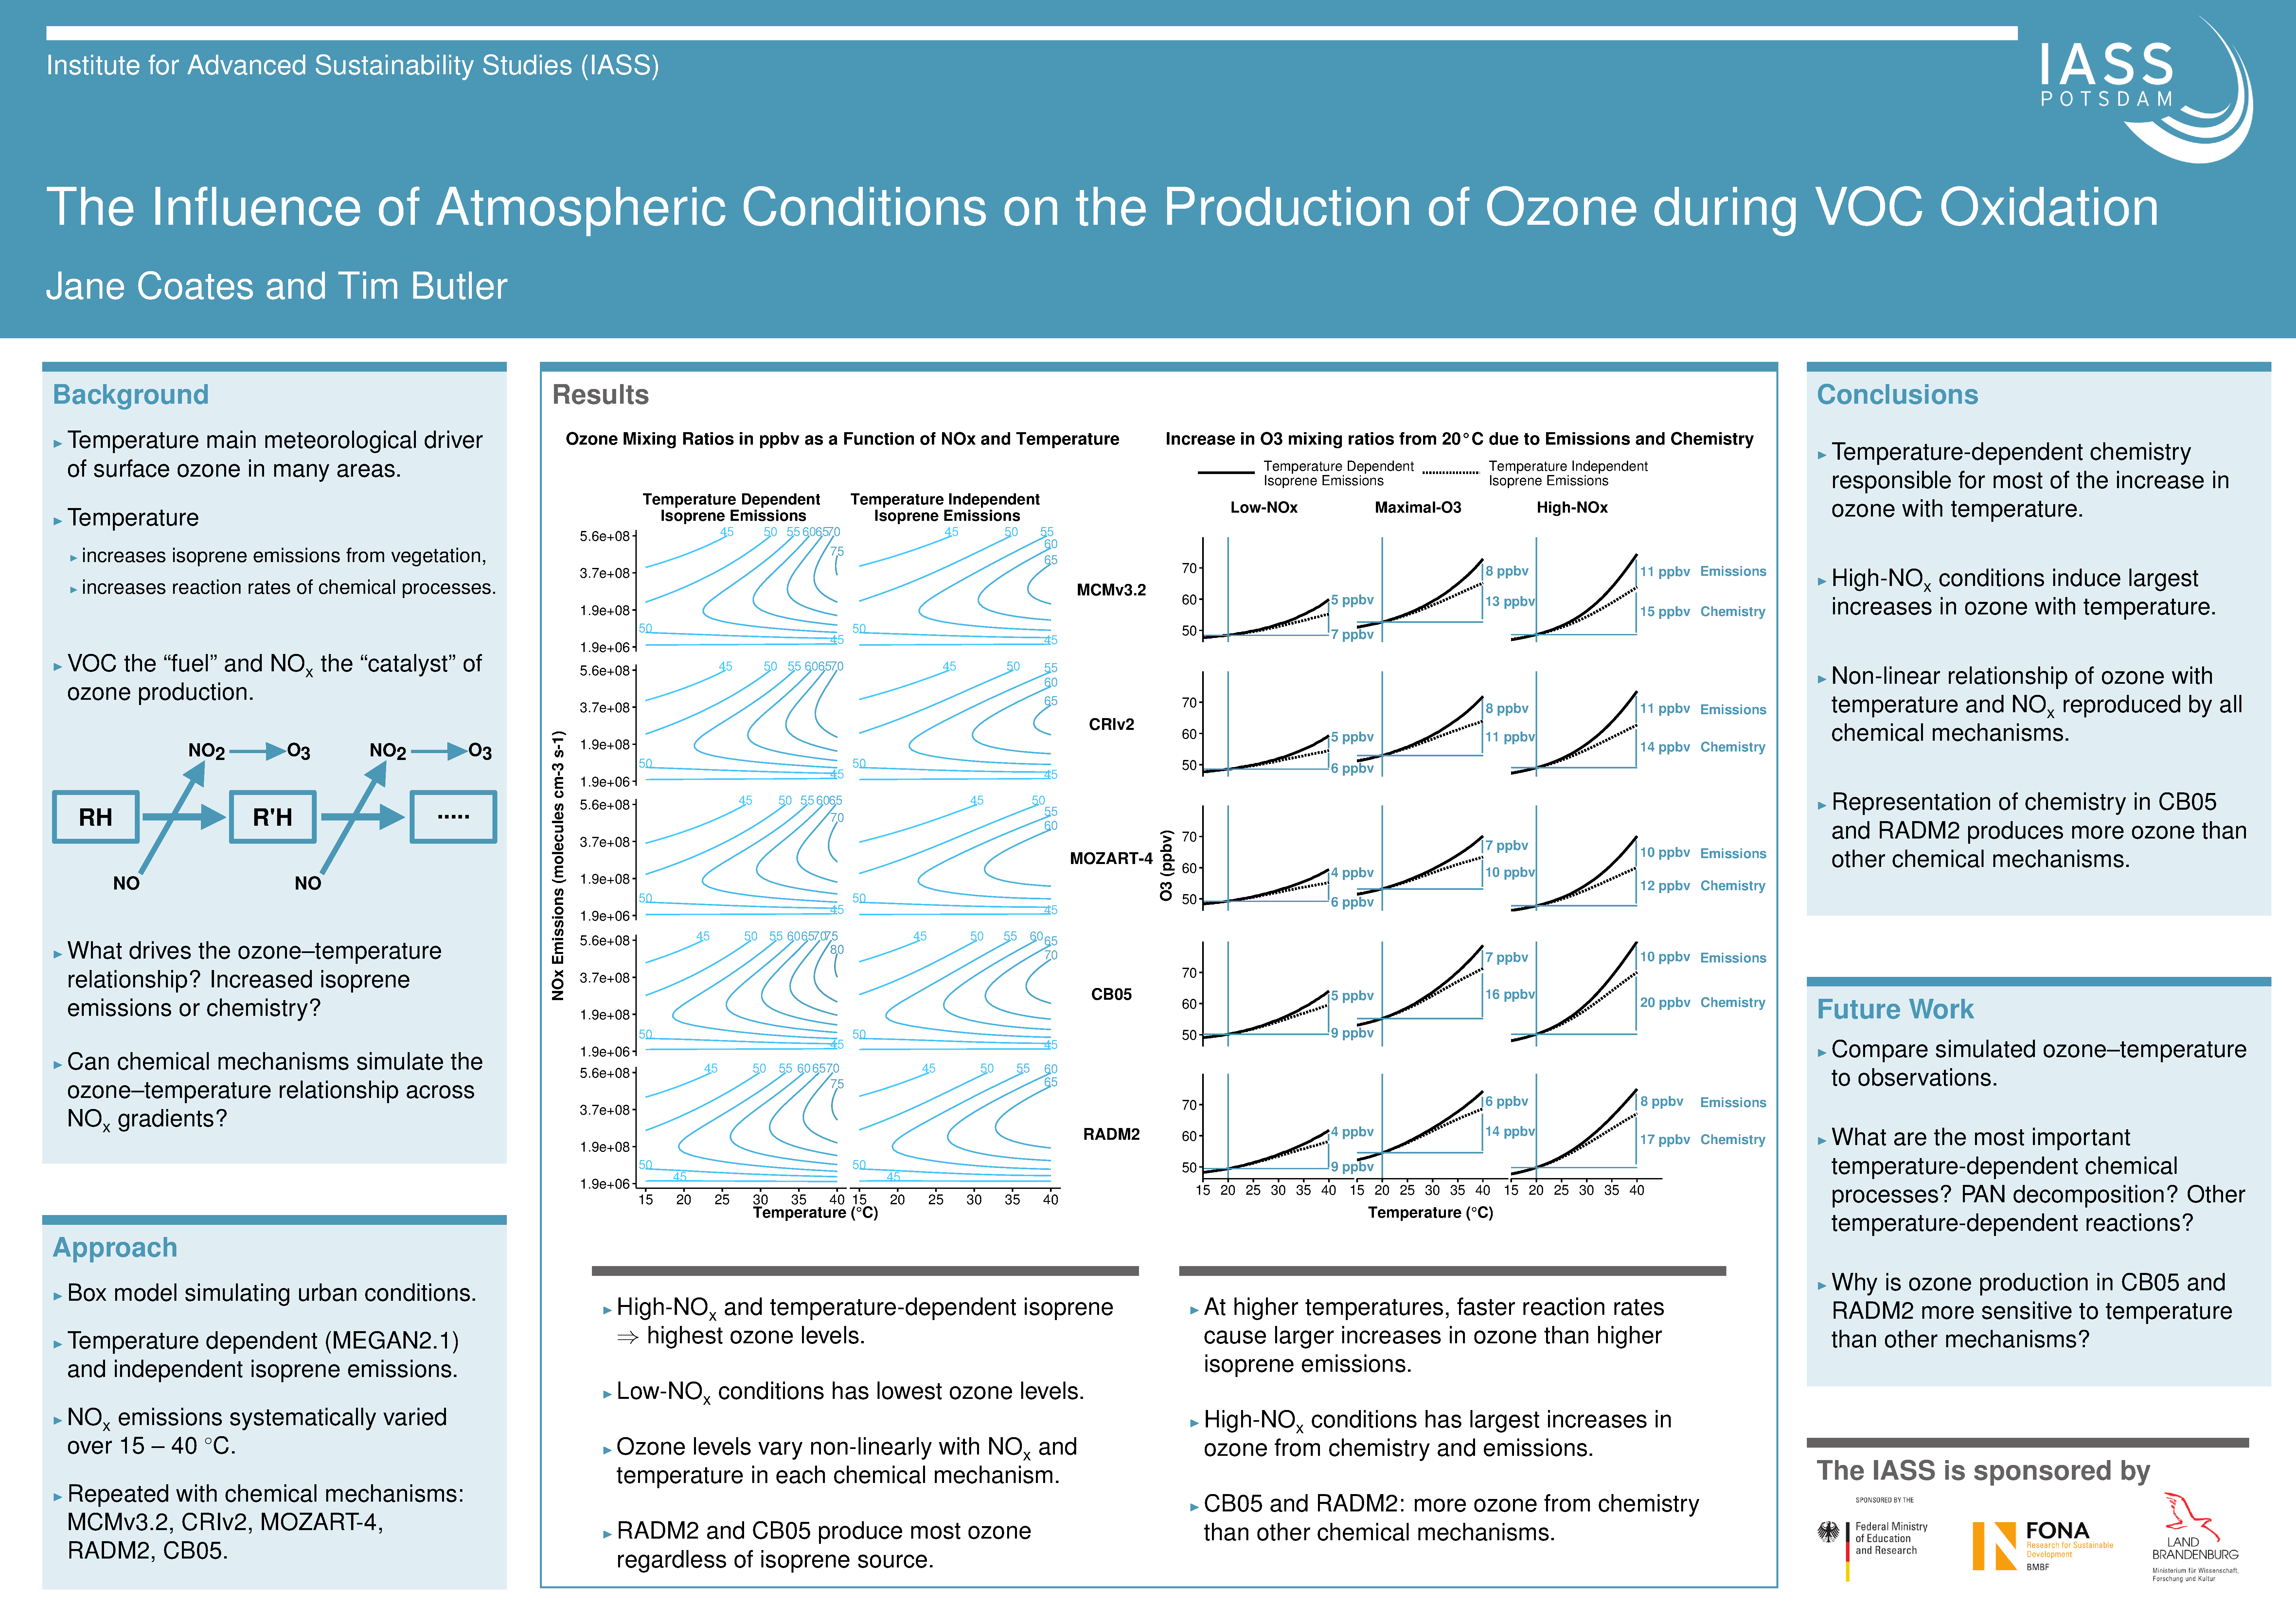
\includegraphics[height = 0.98\paperheight, width = 0.98\paperwidth]{../poster}\hfil}\vfil}
    }
    \begin{frame}[plain]
    \end{frame}
}
\end{document}
